\documentclass[11pt]{article}
\usepackage[textwidth=18.0cm, textheight=23.0cm, top=2.0cm]{geometry}
\usepackage{pst-all}
\usepackage{amssymb}
\usepackage{tikz}
\usepackage{underscore}\begin{document}
\pagestyle{empty}


ClassName: \underline{\textbf{Class_02.2bp-28}}
\par
BinSize: \underline{\textbf{30 × 30}}
\par
ReduceSize: \underline{\textbf{30 × 30}}
\par
TypeNum: \underline{\textbf{48}}
\par
Num: \underline{\textbf{60}}
\par
OutS: \underline{\textbf{1800}}
\par
InS: \underline{\textbf{1737}}
\par
Rate: \underline{\textbf{0.965}}
\par
UB: \underline{\textbf{2}}
\par
LB0: \underline{\textbf{2}}
\par
LB: \underline{\textbf{2}}
\par
LBWithCut: \underline{\textbf{2}}
\par
NodeCut: \underline{\textbf{0}}
\par
ExtendedNodeCnt: \underline{\textbf{1}}
\par
GenNodeCnt: \underline{\textbf{1}}
\par
PrimalNode: \underline{\textbf{0}}
\par
ColumnCount: \underline{\textbf{2}}
\par
TotalCutCount: \underline{\textbf{0}}
\par
RootCutCount: \underline{\textbf{0}}
\par
LPSolverCnt: \underline{\textbf{1}}
\par
PricingSolverCnt: \underline{\textbf{0}}
\par
BranchAndBoundNum: \underline{\textbf{1}}
\par
isOpt: \underline{\textbf{true}}
\par
TimeOnPrimal: \underline{\textbf{0.000 s}}
\par
TimeOnPricing: \underline{\textbf{0.000 s}}
\par
TimeOnRmp: \underline{\textbf{0.078 s}}
\par
TotalTime: \underline{\textbf{0.125 s}}
\par
\newpage


\begin{tikzpicture}[shorten >=1pt,scale=1.0,every node/.style={scale=1.0},->]
\tikzstyle{vertex}=[circle,fill=black!25,minimum size=14pt,inner sep=0pt]
\filldraw[fill=gray!40!white, draw=black] (0,0) rectangle (15.0,15.0);
\foreach \name/\x/\y/\w/\h in {10x10/0.0/0.0/5.0/5.0,10x10/5.0/0.0/5.0/5.0,8x10/0.0/5.0/4.0/5.0,8x10/0.0/10.0/4.0/5.0,10x7/10.0/0.0/5.0/3.5,7x10/4.0/5.0/3.5/5.0,8x8/8.5/5.0/4.0/4.0,8x7/8.5/9.0/4.0/3.5,8x5/8.5/12.5/4.0/2.5,4x10/4.0/10.0/2.0/5.0,10x3/10.0/3.5/5.0/1.5,5x6/12.5/5.0/2.5/3.0,3x9/7.0/10.0/1.5/4.5,5x5/12.5/8.0/2.5/2.5,5x4/12.5/10.5/2.5/2.0,2x10/6.0/10.0/1.0/5.0,2x10/7.5/5.0/1.0/5.0,3x5/12.5/12.5/1.5/2.5,2x5/14.0/12.5/1.0/2.5,3x1/7.0/14.5/1.5/0.5}
\filldraw[fill=white!40!white, draw=black] (\x,\y) rectangle node[draw] (\name) {\name} ++(\w,\h);
\end{tikzpicture}


w =10 , h =10 , x =0 , y =0 , v =100
\par
w =10 , h =10 , x =10 , y =0 , v =100
\par
w =8 , h =10 , x =0 , y =10 , v =80
\par
w =8 , h =10 , x =0 , y =20 , v =80
\par
w =10 , h =7 , x =20 , y =0 , v =70
\par
w =7 , h =10 , x =8 , y =10 , v =70
\par
w =8 , h =8 , x =17 , y =10 , v =64
\par
w =8 , h =7 , x =17 , y =18 , v =56
\par
w =8 , h =5 , x =17 , y =25 , v =40
\par
w =4 , h =10 , x =8 , y =20 , v =40
\par
w =10 , h =3 , x =20 , y =7 , v =30
\par
w =5 , h =6 , x =25 , y =10 , v =30
\par
w =3 , h =9 , x =14 , y =20 , v =27
\par
w =5 , h =5 , x =25 , y =16 , v =25
\par
w =5 , h =4 , x =25 , y =21 , v =20
\par
w =2 , h =10 , x =12 , y =20 , v =20
\par
w =2 , h =10 , x =15 , y =10 , v =20
\par
w =3 , h =5 , x =25 , y =25 , v =15
\par
w =2 , h =5 , x =28 , y =25 , v =10
\par
w =3 , h =1 , x =14 , y =29 , v =3
\par
\newpage


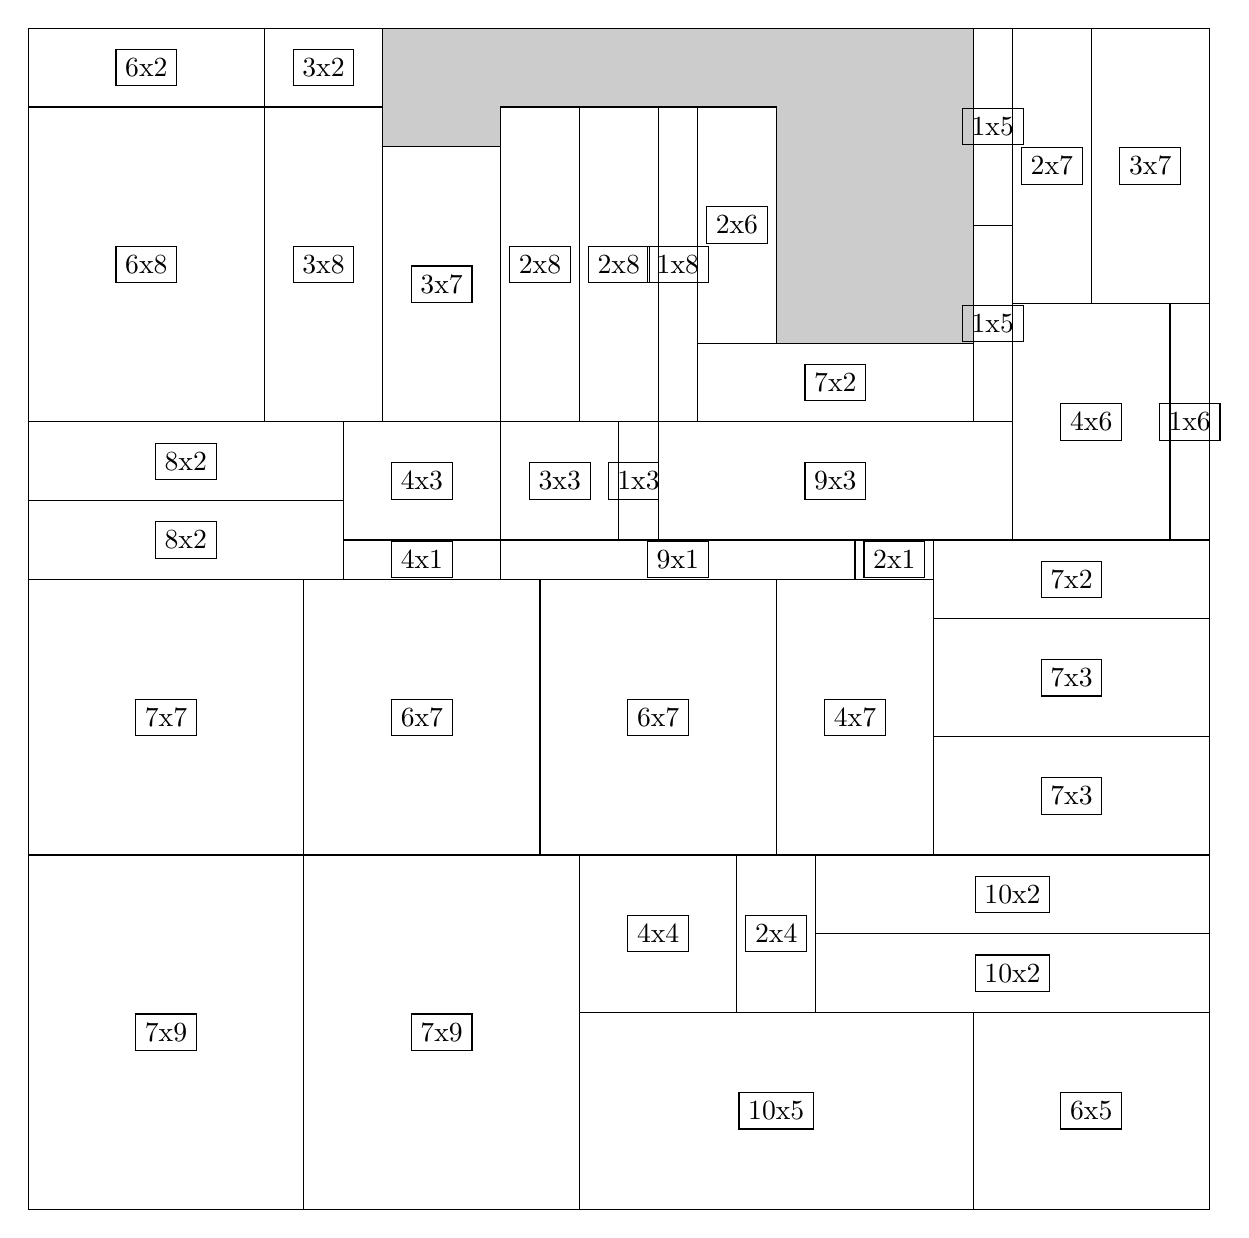
\begin{tikzpicture}[shorten >=1pt,scale=1.0,every node/.style={scale=1.0},->]
\tikzstyle{vertex}=[circle,fill=black!25,minimum size=14pt,inner sep=0pt]
\filldraw[fill=gray!40!white, draw=black] (0,0) rectangle (15.0,15.0);
\foreach \name/\x/\y/\w/\h in {7x9/0.0/0.0/3.5/4.5,7x9/3.5/0.0/3.5/4.5,10x5/7.0/0.0/5.0/2.5,7x7/0.0/4.5/3.5/3.5,6x8/0.0/10.0/3.0/4.0,6x7/3.5/4.5/3.0/3.5,6x7/6.5/4.5/3.0/3.5,6x5/12.0/0.0/3.0/2.5,4x7/9.5/4.5/2.0/3.5,2x1/10.5/8.0/1.0/0.5,4x6/12.5/8.5/2.0/3.0,3x8/3.0/10.0/1.5/4.0,7x3/11.5/4.5/3.5/1.5,7x3/11.5/6.0/3.5/1.5,3x7/13.5/11.5/1.5/3.5,3x7/4.5/10.0/1.5/3.5,10x2/10.0/2.5/5.0/1.0,10x2/10.0/3.5/5.0/1.0,8x2/0.0/8.0/4.0/1.0,8x2/0.0/9.0/4.0/1.0,4x4/7.0/2.5/2.0/2.0,2x8/6.0/10.0/1.0/4.0,2x8/7.0/10.0/1.0/4.0,7x2/11.5/7.5/3.5/1.0,7x2/8.5/10.0/3.5/1.0,2x7/12.5/11.5/1.0/3.5,6x2/0.0/14.0/3.0/1.0,4x3/4.0/8.5/2.0/1.5,2x6/8.5/11.0/1.0/3.0,9x1/6.0/8.0/4.5/0.5,3x3/6.0/8.5/1.5/1.5,2x4/9.0/2.5/1.0/2.0,1x8/8.0/10.0/0.5/4.0,3x2/3.0/14.0/1.5/1.0,1x6/14.5/8.5/0.5/3.0,1x5/12.0/10.0/0.5/2.5,1x5/12.0/12.5/0.5/2.5,4x1/4.0/8.0/2.0/0.5,1x3/7.5/8.5/0.5/1.5,9x3/8.0/8.5/4.5/1.5}
\filldraw[fill=white!40!white, draw=black] (\x,\y) rectangle node[draw] (\name) {\name} ++(\w,\h);
\end{tikzpicture}


w =7 , h =9 , x =0 , y =0 , v =63
\par
w =7 , h =9 , x =7 , y =0 , v =63
\par
w =10 , h =5 , x =14 , y =0 , v =50
\par
w =7 , h =7 , x =0 , y =9 , v =49
\par
w =6 , h =8 , x =0 , y =20 , v =48
\par
w =6 , h =7 , x =7 , y =9 , v =42
\par
w =6 , h =7 , x =13 , y =9 , v =42
\par
w =6 , h =5 , x =24 , y =0 , v =30
\par
w =4 , h =7 , x =19 , y =9 , v =28
\par
w =2 , h =1 , x =21 , y =16 , v =2
\par
w =4 , h =6 , x =25 , y =17 , v =24
\par
w =3 , h =8 , x =6 , y =20 , v =24
\par
w =7 , h =3 , x =23 , y =9 , v =21
\par
w =7 , h =3 , x =23 , y =12 , v =21
\par
w =3 , h =7 , x =27 , y =23 , v =21
\par
w =3 , h =7 , x =9 , y =20 , v =21
\par
w =10 , h =2 , x =20 , y =5 , v =20
\par
w =10 , h =2 , x =20 , y =7 , v =20
\par
w =8 , h =2 , x =0 , y =16 , v =16
\par
w =8 , h =2 , x =0 , y =18 , v =16
\par
w =4 , h =4 , x =14 , y =5 , v =16
\par
w =2 , h =8 , x =12 , y =20 , v =16
\par
w =2 , h =8 , x =14 , y =20 , v =16
\par
w =7 , h =2 , x =23 , y =15 , v =14
\par
w =7 , h =2 , x =17 , y =20 , v =14
\par
w =2 , h =7 , x =25 , y =23 , v =14
\par
w =6 , h =2 , x =0 , y =28 , v =12
\par
w =4 , h =3 , x =8 , y =17 , v =12
\par
w =2 , h =6 , x =17 , y =22 , v =12
\par
w =9 , h =1 , x =12 , y =16 , v =9
\par
w =3 , h =3 , x =12 , y =17 , v =9
\par
w =2 , h =4 , x =18 , y =5 , v =8
\par
w =1 , h =8 , x =16 , y =20 , v =8
\par
w =3 , h =2 , x =6 , y =28 , v =6
\par
w =1 , h =6 , x =29 , y =17 , v =6
\par
w =1 , h =5 , x =24 , y =20 , v =5
\par
w =1 , h =5 , x =24 , y =25 , v =5
\par
w =4 , h =1 , x =8 , y =16 , v =4
\par
w =1 , h =3 , x =15 , y =17 , v =3
\par
w =9 , h =3 , x =16 , y =17 , v =27
\par
\newpage


\end{document}